\documentclass[../summary.tex]{subfiles}

\begin{document}
	
	\section{Energy}
	
	\subsection{Study guide}
	\begin{itemize} 
		\setlength{\itemsep}{0pt}
		
		\item What is energy?
		\begin{itemize}
			\item Understanding the meaning of the first and second law of thermodynamics in energy production
			\item Knowing the concepts of energy, power, energy vectors, energy balances and energy systems
		\end{itemize}
		
		\item Thermic energy sources
		\begin{itemize}
			\item Recognizing primary and secondary sources of energy
			\item Understanding the link between energy production and climate change
			\item Knowing the principles of combined cycle power (CCPP) and combined heat and power (CHP)
			\item Having an idea of orders of magnitude and efficiency of the different production technologies
			\item Knowing the different types of gas used in the energy system
		\end{itemize}
		
		\item Renewable energy sources
		\begin{itemize}
			\item Understanding the basic principles of renewable energy production
		\end{itemize}
		
		\item Energy cost
		\begin{itemize}
			\item Knowing the concepts LCOE, dunkleflaute and duck-curve
			\item Understanding the consequences of unbalances between production and consumption
		\end{itemize}
		
		\item Energy networks
		\begin{itemize}
			\item Understanding the difference between the meshed high voltage grids and local radial 
			
			distribution grids
			\item Understanding the added value of adding a communication layer to the energy networks
		\end{itemize}
		
		\item Energy efficiency
		\begin{itemize}
			\item Having an idea of the relative parts of industry, transport and built environment in energy consumption
			\item Understanding the direct and indirect rebound effects of energy saving measures
		\end{itemize}
		
		\item Energy consumption
		\begin{itemize}
			\item Understanding how the energy consumption can be organized more sustainable
			\item What might be the role of hydrogen?
		\end{itemize}
		
		\item Energy storage
		\begin{itemize}
			\item Understanding the key role of lithium batteries in the energy transition
			\item Knowing different storage technologies
		\end{itemize}
		
		\item Energy markets
		\begin{itemize}
			\item Understanding the difference between old and new tarriff schemes for energy
		\end{itemize}
		
		\item Energy policies
		\begin{itemize}
			\item What is the emission trading system?
		\end{itemize}
	\end{itemize}
	\newpage
	\subsection{What is energy?}
	
	\textbf{Energy} is what causes change in the physical sense: for instance, you can do work or heat something up, or cause a chemical reaction. Energy is expressed in Joules [J]. When we want to explain how much energy is converted per time unit, we talk of \textbf{power}, expressed in Watt (Joules per second).In many practical applications the unit kWh is used: this is the amount of energy converted by an application with a power of 1 kW, if it would run for 1 hour. \textbf{Energy vectors} can be defined as the forms of energy, for example heat present in warm water or steam, electricity and chemical energy.
	\\\\
	In principle, energy cannot be destroyed nor created, it will always be converted in some other form. These conversions will not always be useful or desired. This is know as the \textbf{first law of thermodynamics}. Furthermore, some energy conversions can happen in the two directions: think of the battery in your mobile phone that can be charged and later discharged. Other conversions can only happen in one direction, for instance, you can burn a fuel to run a combustion engine in a car resulting in kinetic or motion energy, but you cannot recover the fuel as such when you slow down again. This follows from the \textbf{second law of thermodynamics}.
	\\\\
	Engineers usually talk about an \textbf{energy system}. This can be your home: you import energy like electricity or gas, to be converted into an energy service or end-use like lighting or heating. This is a simple example of an \textbf{energy balance}. The amount of energy that is consumed equals the imported energy, of course plus some losses. When we zoom out, such energy balances can be drawn up for an entire country: typically, oil or gas, or perhaps coal is imported.
	
	\subsection{Thermic energy sources}
	
	\textbf{Primary energy sources} are found in nature in a stable form: for instance, oil, coal or sun light. \textbf{Secondary energy sources} do not occur in a stable natural form, but are created by conversion of a primary source. Electricity or hydrogen, so-called energy vectors, belong to this category. They might exist in nature – think of a lightning strike – but are not stable or concentrated enough to be usable.
	\\\\
	Some of these energy sources are renewable. Fossil fuels are not. These \textbf{fossil fuels}, typically in the form of coal, oil or gas, could lead to sustainability issues. Combusting them rises the CO2-levels in the atmosphere, thereby \textbf{contributing to climate change}. 
	\\\\
	The laws of thermodynamics will tell that the \textbf{conversion from energy sources into a usable form}, think of refined fuel such as gasoline or electricity, \textbf{will generate losses}. As a consequence, the total \textbf{efficiency is less than 40\%}, meaning the majority of the primary energy is turned into useless heat rather than electricity. Gas power plants look pretty much the same. However, the modern ones are so-called \textbf{Combined Cycle Power Plants (CCPP)}. They first use a compressor-combustion chamber-turbine combination which is similar to aircraft engines, but then with an electrical generator attached. The exhaust gases are hot enough to pass through a boiler after which electricity is generated with the steam cycle. The combination of these two machine sets lifts the \textbf{total efficiency up to 55 to 60\%}. An additional benefit is that these are much more dynamic and can change their output power rapidly. 
	\\
	\\
	Such combined cycles are used in other applications as well, under the name \textbf{Combined Heat and Power systems (CHP)}: for instance, many industrial processes in the food or chemical industry need a lot of high-temperature heat. By combine an electricity generation cycle with an exhaust temperature close to the process temperature, a \textbf{very high total efficiency} can be obtained.
	\\\\
	The \textbf{traditionally used gas} in these conversions is natural gas, containing fossil-based \textbf{methane originating from gas fields}. This methane can be extracted \textbf{from rocky layers}, but also \textbf{from biological processes} like fermentation, of for instance \textbf{specifically grown plants or organic waste}, coming from agriculture, food industry, etc. Finally, gas \textbf{can be made synthetically through a chemical process} starting from hydrogen and a carbon source.
	
	\subsection{Renewable energy sources}
	
	It is possible to convert \textbf{direct or scattered sun light} directly into electricity using so-called \textbf{photovoltaic}, in short “PV”, \textbf{cells}. Another form of weather-driven electricity production uses \textbf{wind} to drive large free-standing \textbf{turbines} with a build-in electricity generator. For completeness, we should also mention \textbf{hydropower}-based electricity production, which is in principle operating renewable and carbon-emission free as well. This kind of power plants use giant \textbf{dams} to withhold water on a river or a large difference in height in a mountainous region. By releasing the water through a turbine-generator combination, electricity is produced.
	
	\subsection{Energy cost}
	
	To make a fair comparison between the costs before and after the construction phase, the so-called \textbf{Levelized Cost Of Electricity (LCOE)} can be used. This allows to include all these costs over the whole lifetime of the installation on a common basis and average them over the produced unit of electrical energy. It can be noted that \textbf{most technology become cheaper when they mature}, the so-called learning curve. This can be seen in figure \ref{fig:lcoe}.
	
	\begin{figure}[H]
		\centering
		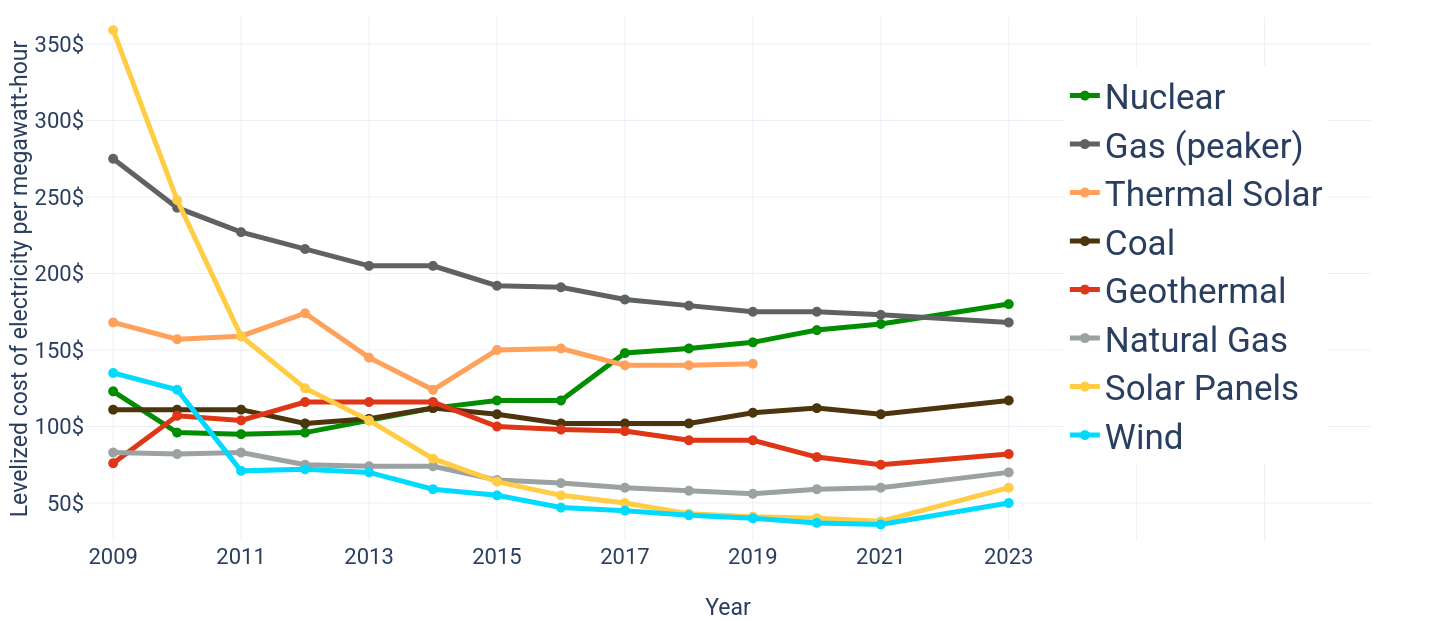
\includegraphics[width=0.75\linewidth]{../images/4-LCOE}
		\caption{Levelized cost of electricity over the most recent years}
		\label{fig:lcoe}
	\end{figure}
	
	\ \\
	In a system with many weather-related renewable sources like solar power, there is an obvious difference between the middle of the day, when there is abundant sun and the night. Because of the unbalances between production and consumption, the transition in between asks for a lot of alternative power sources to come on line. These can be batteries, other controlled power plants, or exchanges over the electricity grid with connected regions. This is depicted in the so-called \textbf{Duck Curve} (figure \ref{fig:duck-curve}). 
	
	\begin{figure}[H]
		\centering
		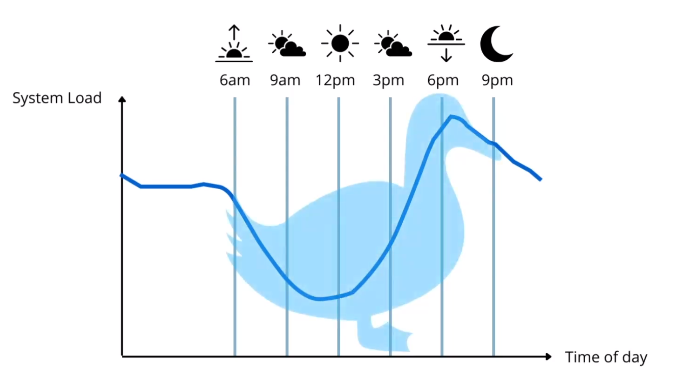
\includegraphics[width=0.6\linewidth]{../images/4-duck-curve}
		\caption{Duck Curve}
		\label{fig:duck-curve}
	\end{figure}
	
	\ \\
	If we zoom out over a series of days, we have to account for cloudy days with for instance less wind. These are often referred to as \textbf{Dunkelflaute}, a German word. In practice also here the solution is a mix of generation technologies and international energy exchanges.
	
	\subsection{Energy networks}
	
	For the transportation of energy between end consumers, networks are needed. At the highest level, you find the electrical transmission grids. This can be in the form of \textbf{high voltage lines}, underground cables or even cables through the bottom of the sea. When you look at the map of a high voltage system, you will see that \textbf{these lines form large meshes}. Every substation is connected through multiple high-volt slides.This is done \textbf{to increase the reliability}. 
	\\\\
	At a more local level, you will find the \textbf{local distribution grid}. In most countries, this is built with a system of underground cables under the streets. Contrary to the high voltage grid, the topology here is \textbf{radial}. In the distribution grid, multiple voltages are used. In the last part closest to your home, a transformer will step down the voltage to a safe level, which can be brought inside your house. 
	\\\\
	These days, it is almost impossible to run all those \textbf{energy networks} without digital tools for \textbf{management or protection}. Therefore, the \textbf{presence of a dependable communication system is a necessity}. In fact, the whole energy system is a so-called system of systems.
	
	\subsection{Energy efficiency}
	
	In most European countries, roughly \textbf{1/3 of the energy} will be \textbf{consumed in industry} and \textbf{1/3} is \textbf{needed for transportation}. The \textbf{rest} is \textbf{used in the build environment}, for energy services like heating and lighting. 
	\\\\
	When we consider energy consumption we want this to be as efficient as possible. Unfortunately replacing an energy-consuming device with one that is, as an example, 10 times more efficient, will not result in an overall 10 times lower energy consumption. The explanation for this is found in the so-called \textbf{rebound effects}: when you give people a more efficient device for instance and a led lamp, they tend to let it burn longer, compensating about 20\% of the possible savings. This is the so-called \textbf{direct rebound}. There is also an \textbf{indirect rebound}, accounting for about 10\% of the possible savings, which is explained by the fact that you will save money which you spent on other energy consuming goods.  This is visualized in figure \ref{fig:rebound-effects}.
	
	\begin{figure}[H]
	\centering
	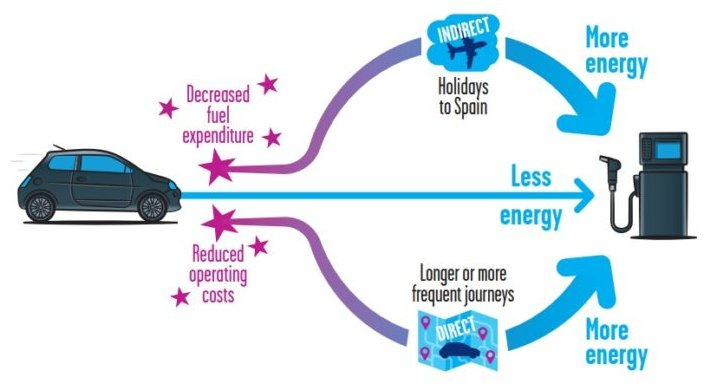
\includegraphics[width=0.7\linewidth]{../images/4-rebound-effects}
	\caption{The Rebound Effects}
	\label{fig:rebound-effects}
\end{figure}
	
	\subsection{Energy consumption}
	
	There are multiple ways the energy consumption can be organized more sustainable. For instance, there are more and more \textbf{photovoltaic panels} on our buildings. This means we can produce a lot of electricity locally and store the excess of produced energy in home batteries. Furthermore, newly available technology like the \textbf{heat pump} is a much more effective way to heat buildings. When using heat pumps, 3 to 5 times less energy is needed and CO2 emissions will be reduced significantly. The rise of electric vehicles in favour of fossil fuel driven cars also results in more sustainability.
	\\\\
	When we look at the usage of natural gas and fossil fuels, we might consider dropping them and using a more sustainable alternative like \textbf{hydrogen} instead. However, the problem with  hydrogen is that it needs \textbf{a lot of consecutive conversions} to produce it and make it usable for the end consumer. Because of the conversions, there are \textbf{a lot of losses over the whole chain of processes}. This makes the hydrogen route \textbf{5 to 6 times less efficient} than the direct electric route with heat pumps. Therefore, this isn't a suitable alternative at the moment, except for long distance transport, such as long range shipping or airplanes.
	
	\subsection{Energy storage}
	
	Although batteries already exist for many decades, one could say that the relatively recent \textbf{lithium battery should be considered as a key enabler of the energy transition}. Mass production of batteries brought down the price of lithium batteries with a factor of 10 in the last decade. Such lithium based batteries have the advantage that they \textbf{can be charged and discharged hundreds even thousands of times without significant reduction in capacity}. They are also very compact and have therefore \textbf{high energy and power density}. Lastly, modern types of lithium batteries are also \textbf{fully recyclable} and don't contain cobalt anymore. 
	\\\\
	Batteries are a great solution to balance production and demand of electricity over a relatively short term being within a day or over the course of a week. However to balance energy over a longer period, for instance, between seasons, \textbf{other forms of energy storage} are needed. For this purpose, \textbf{thermal storage} or \textbf{pumped hydro storage using large water basins} are applicable. 
	
	\subsection{Energy markets}
	
	\textbf{ Since the turn of the century}, in Europe, the electricity and gas market, evolved towards a so-called “free” market, with \textbf{energy prices} being\textbf{ determined by offer and demand within a market system, rather than fixed up front}. In the past we just paid for the energy consumed: the kilowatt hours of electricity, the liters of fuel or the cubic metres of gas. However, this is changing.
	\\\\
	With the availability of renewable energy sources like sun or wind, which are produced at almost no production cost, it is mainly the investments that are driving the price. In addition, the energy grids, more in particular the electricity grid, are stressed much more. Therefore, \textbf{the newer electricity tariffs are rather driven by the capital costs than the operational costs}, and we see a \textbf{shift from bills based upon kilowatt hours to capacity-based charging}. 
	
	\subsection{Energy policies}
	
	A series of European directives have been developed: they form the basis of the energy markets, set the goals for energy efficiency measures, and the decarbonization. 
	\\\\
	The \textbf{emission trading system (ETS)} is an example of this. The idea behind this is to award tradeable rights to emit CO2 and to set clear goals to significantly reduce this by the middle of the century. In this way the technologies that can mitigate CO2 emissions in the most economic way will be favoured. In practice this works like a carbon tax, which is included in the price of electricity or industrial products.
	
\end{document}
